%%%%%%%%%%%%%%%%%%%%%%%%%%%%%%%%%%%%%%%%%%%%%%%%%%%%%%%%%%%%%%%%%%%%%%%%%%%%%%%
% The Mathematical Model of the Point: A Dynamical Spacetime Framework 
% for Black-Hole Interiors
% Author: Xiaohui Li
% This LaTeX file is self-contained and compiles with pdflatex.
%%%%%%%%%%%%%%%%%%%%%%%%%%%%%%%%%%%%%%%%%%%%%%%%%%%%%%%%%%%%%%%%%%%%%%%%%%%%%%%

\documentclass[11pt,a4paper]{article}

\usepackage[utf8]{inputenc}
\usepackage[T1]{fontenc}
\usepackage{amsmath,amssymb,amsfonts}
\usepackage{graphicx}
\usepackage{geometry}
\usepackage{setspace}
\usepackage{natbib}
\usepackage{hyperref}
\usepackage{tikz}
\usepackage{pgfplots}
\pgfplotsset{compat=1.18}
\usetikzlibrary{shapes.geometric, arrows.meta, positioning, calc}

\geometry{left=2.5cm,right=2.5cm,top=2.5cm,bottom=2.5cm}

\title{\bfseries The Mathematical Model of the Point:\\
A Dynamical Spacetime Framework for Black-Hole Interiors}

\author{Xiaohui Li$^{*}$\\
\normalsize Independent Researcher, 721000 Baoji, China\\
\normalsize $^{*}$Correspondence: danceluck@163.com; ORCID: 0009-0003-8233-7191}

\date{}

\begin{document}

\maketitle

\begin{abstract}
\noindent
We propose the Dynamical Point Model (DPM), a theoretical framework in which a physical point is not a static, zero-dimensional Euclidean object but an irreducible quantum-geometric cell endowed with internal structure. By introducing a chiral-quantum mixing field as the primordial generator of dimensionality, we show that the Schwarzschild singularity can be regularized into a finite, generative spacetime core. Hierarchical cosmic seeds---particles, stars, and black holes---are unified as successive stages of chiral aggregation. The model predicts measurable gravitational-wave echoes, a characteristic primordial black-hole mass spectrum, and high-energy cosmic-ray spectral anomalies. We report proof-of-concept numerical simulations and outline benchmark tests against LIGO/Virgo/KAGRA gravitational-wave data, Planck cosmic microwave background constraints, and future event-horizon substructure observations.
\end{abstract}

\noindent\textbf{Keywords:} black hole interior; quantum geometry; chiral quantum mixing; singularity resolution; cosmic seeds; gravitational-wave echoes; dynamical point; hierarchical seed model

\section{Introduction}

The standard interpretation of the Schwarzschild solution treats the central singularity ($r = 0$) as the inevitable temporal endpoint of all infalling matter, beyond which no classical spacetime exists \cite{schwarzschild1916,oppenheimer1939}. Penrose and Hawking proved that such singularities are generic consequences of classical general relativity under plausible energy conditions \cite{penrose1965,hawking1966}. Yet the very existence of a curvature singularity signals the breakdown of the theory itself, motivating a long-standing search for ultraviolet completions in loop quantum gravity, string theory, and non-singular black-hole models \cite{bardeen1968,hayward2006,ashtekar2006,rovelli2014,maldacena1998}.

An alternative intuition, articulated in preliminary form by Li \cite{li2024}, holds that a black hole is not merely a dead end but a cosmic seed: a finite, structured object whose interior hosts a new spacetime region. In this view, physical points possess internal structure, dimensions are dynamically generated by chiral-quantum mixing, and the Universe consists of a nested hierarchy of seeds---particles, stars, black holes, and galaxies \cite{li2024}. Although such a picture appears to conflict with the Schwarzschild singularity theorem, we argue here that the conflict is only apparent: the singularity theorems constrain classical geometry, whereas the DPM describes a quantum-geometric regularization of the endpoint.

The present paper formalizes these intuitions into a mathematically consistent model. We distinguish between a Euclidean mathematical point---a coordinate label with no extension---and a physical point, which carries a minimal quantum volume and an internal state. We then construct a regular black-hole metric inspired by Hayward's nonsingular solution \cite{hayward2006} and interpret its de-Sitter-like core as the ``internal universe.'' We derive falsifiable predictions, describe numerical simulations, and discuss how the framework can be benchmarked against existing data.

\section{The Hierarchical Cosmic Seed Framework}

Observations show that the Universe is overwhelmingly composed of hydrogen, the simplest atom \cite{draine2011}. In the DPM, hydrogen atoms are interpreted as first-level cosmic seeds: stable chiral aggregates that generate the entire chemical periodic table through nucleosynthesis and stellar evolution. When first-level seeds gravitationally assemble, they form second-level seeds---stars. Stellar evolution then produces third-level seeds---black holes---which in turn coalesce into supermassive black holes at galactic centers \cite{kormendy2013}. The formation of the first same-handed chiral state marks the onset of this hierarchical aggregation; mutual attraction between like-chiral quanta drives condensation, while residual mixing supplies the perturbations required for structure formation.

Mathematically, we describe the hierarchy by a sequence of effective actions:
\begin{equation}
S_n = \int d^4x \sqrt{-g} \left[ \frac{R}{16\pi G} + \mathcal{L}_\chi^{(n)} + \mathcal{L}_{\rm matter}^{(n)} \right], \quad n = 1, 2, 3, \ldots
\label{eq:action}
\end{equation}
where $\mathcal{L}_\chi^{(n)}$ denotes the chiral-mixing Lagrangian at seed level $n$. Each level inherits an effective coupling constant $g_n$ that decreases as the seed mass increases, reflecting the successive symmetry breakings of the chiral field.

% Figure 1
\begin{figure}[htbp]
\centering
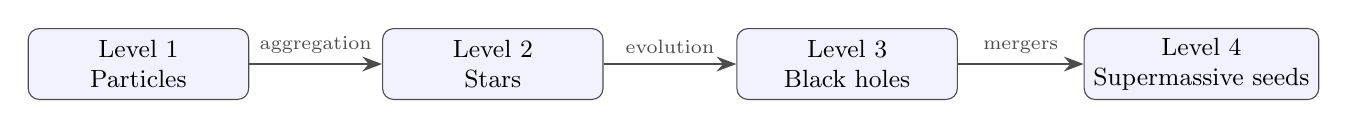
\begin{tikzpicture}[
    box/.style={rectangle, rounded corners, draw=black!70, fill=blue!5, minimum width=2.8cm, minimum height=0.9cm, align=center, font=\small},
    arrow/.style={-{Stealth[length=2.5mm]}, thick, black!70}
]
\node[box] (p) at (0,0) {Level 1\\Particles};
\node[box] (s) at (4.5,0) {Level 2\\Stars};
\node[box] (bh) at (9,0) {Level 3\\Black holes};
\node[box] (sm) at (13.5,0) {Level 4\\Supermassive seeds};
\draw[arrow] (p) -- (s) node[midway,above,font=\scriptsize] {aggregation};
\draw[arrow] (s) -- (bh) node[midway,above,font=\scriptsize] {evolution};
\draw[arrow] (bh) -- (sm) node[midway,above,font=\scriptsize] {mergers};
\end{tikzpicture}
\caption{\textbf{Hierarchical cosmic seed structure.} First-level seeds (particles such as hydrogen atoms) combine to form second-level seeds (stars); stellar evolution produces third-level seeds (black holes); black holes merge into supermassive seeds at galactic centres. Chiral-quantum mixing drives aggregation at every level.}
\label{fig:seeds}
\end{figure}

\section{From Mathematical Point to Physical Point: A Dynamical Geometry}

Euclidean geometry defines a point as ``that which has no part'' \cite{euclid}: a zero-dimensional object with neither length, area, nor volume. A line is the locus of a point in motion, not a concatenation of static points. In classical mathematics, this abstraction is consistent because points are mere coordinates.

The DPM rejects the identification of a physical point with a Euclidean point. Quantum mechanics, supported by Heisenberg uncertainty and the existence of vacuum fluctuations \cite{casimir1948}, implies that any physical localization event is accompanied by an irreducible minimal scale. We therefore endow each physical point $P$ with an internal Hilbert-space state $|\psi_P\rangle$ and a characteristic length $\ell_P = \alpha \ell_{\rm Pl}$, where $\ell_{\rm Pl} = \sqrt{\hbar G/c^3}$ is the Planck length and $\alpha$ is a dimensionless parameter expected to be of order unity.

The generation of dimensions is modelled by a chiral-quantum mixing field $\chi(x)$ with a double-well potential:
\begin{equation}
V(\chi) = \lambda (\chi^2 - \eta^2)^2.
\label{eq:potential}
\end{equation}
When $\chi$ settles into one of the two minima $\pm\eta$, a definite chiral state is selected. A small mixing perturbation $\delta\chi$ transverse to the vacuum manifold acts as a displacement operator that promotes a 0-dimensional point to a 1-dimensional line element; a second orthogonal perturbation generates a 2-dimensional surface; a third generates a 3-volume; and additional perturbations generate higher-dimensional structures. This construction justifies the statement that ``mathematics should be dynamic'': dimensionality is not given a priori but is generated by the temporal evolution of the chiral field.

% Figure 2 -- FIXED LAYOUT
\begin{figure}[htbp]
\centering
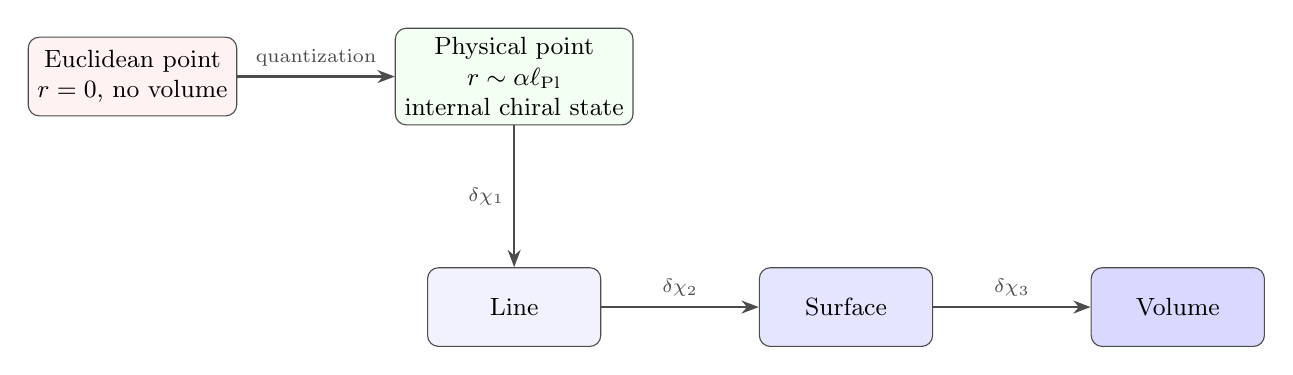
\begin{tikzpicture}[
    box/.style={rectangle, rounded corners, draw=black!70, minimum width=2.2cm, minimum height=1.0cm, align=center, font=\small},
    arrow/.style={-{Stealth[length=2.2mm]}, thick, black!70},
    node distance=1.8cm and 2.0cm
]
% Top row: Euclidean -> Physical point
\node[box, fill=red!5] (a) {Euclidean point\\$r=0$, no volume};
\node[box, fill=green!5, right=of a] (b) {Physical point\\$r \sim \alpha \ell_{\rm Pl}$\\internal chiral state};
\draw[arrow] (a) -- (b) node[midway,above,font=\scriptsize] {quantization};

% Bottom row: Physical point -> dimensions
\node[box, fill=blue!5, below=of b] (c) {Line};
\node[box, fill=blue!10, right=of c] (d) {Surface};
\node[box, fill=blue!15, right=of d] (e) {Volume};
\draw[arrow] (b) -- (c) node[midway,left,font=\scriptsize] {$\delta\chi_1$};
\draw[arrow] (c) -- (d) node[midway,above,font=\scriptsize] {$\delta\chi_2$};
\draw[arrow] (d) -- (e) node[midway,above,font=\scriptsize] {$\delta\chi_3$};
\end{tikzpicture}
\caption{\textbf{From mathematical point to physical point.} (a) The Euclidean point is a static coordinate with no extension. (b) The physical point carries a minimal quantum volume and an internal chiral state; perturbations of the chiral field dynamically generate line, surface, volume, and higher-dimensional structures.}
\label{fig:point}
\end{figure}

\section{A Regular Interior Metric and the Birth of an Internal Universe}

To implement a physical point at the black-hole centre, we adopt a regular metric of the form
\begin{equation}
ds^2 = -f(r)\,dt^2 + f(r)^{-1}\,dr^2 + r^2\,d\Omega^2,
\label{eq:metric}
\end{equation}
with
\begin{equation}
f(r) = 1 - \frac{2GM r^2}{r^3 + 2GM r_c^2}.
\label{eq:fr}
\end{equation}
Here $r_c = \alpha \ell_{\rm Pl}$ is the core radius, and Eq.~(\ref{eq:fr}) is a one-parameter generalization of Hayward's nonsingular black-hole solution \cite{hayward2006}. The effective interior mass is
\begin{equation}
M(r) = \frac{M r^3}{r^3 + 2GM r_c^2},
\label{eq:mass}
\end{equation}
so that $M(0)=0$ and $M(r)\to M$ as $r\to\infty$. At the centre, $f(0)=1$, and the Kretschmann scalar $K = R_{\mu\nu\rho\sigma}R^{\mu\nu\rho\sigma}$ remains finite:
\begin{equation}
K(0) = \frac{48 G^2 M^2}{r_c^6}.
\label{eq:kretschmann}
\end{equation}

For $r \ll r_c$, the metric approximates a de Sitter geometry:
\begin{equation}
f(r) \approx 1 - \frac{r^2}{r_c^2},
\label{eq:desitter}
\end{equation}
with an effective cosmological constant
\begin{equation}
\Lambda_{\rm eff} = \frac{3}{r_c^2} \sim \frac{3}{\alpha^2 \ell_{\rm Pl}^2}.
\label{eq:lambda}
\end{equation}
Thus the central region is not a singular point but a finite, causally regular spacetime---an ``internal universe'' born from the chiral-quantum core. This is the precise sense in which a black hole contains a new spacetime.

% Figure 3
\begin{figure}[htbp]
\centering
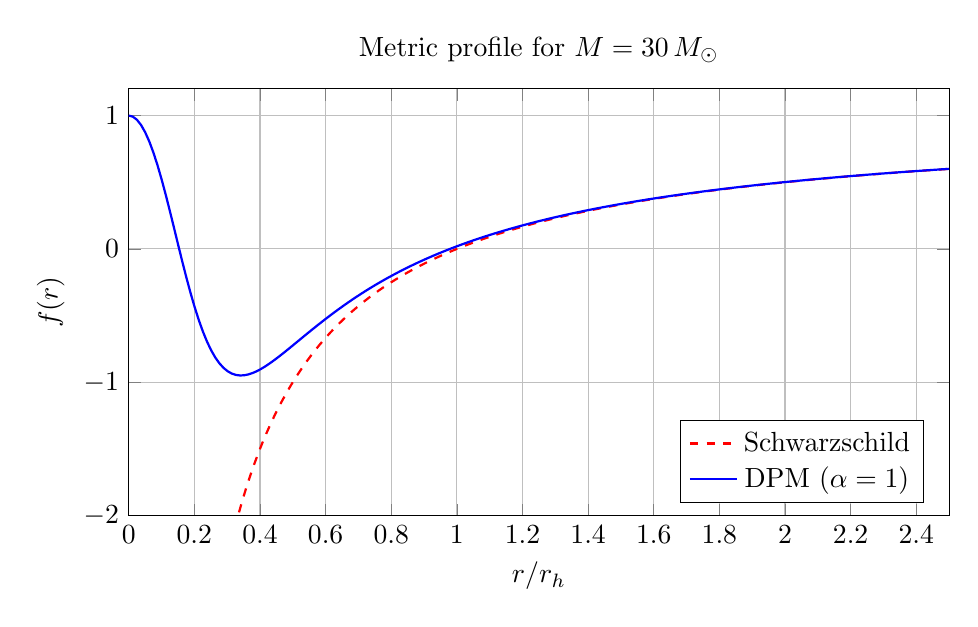
\begin{tikzpicture}
\begin{axis}[
    width=12cm, height=7cm,
    xlabel={$r / r_h$},
    ylabel={$f(r)$},
    xmin=0, xmax=2.5,
    ymin=-2, ymax=1.2,
    legend pos=south east,
    grid=major,
    title={Metric profile for $M = 30\,M_\odot$}
]
\addplot[domain=0.05:2.5, samples=200, thick, dashed, red] {1 - 1/x};
\addplot[domain=0:2.5, samples=200, thick, blue] {1 - (x^2)/(x^3 + 0.02)};
\legend{Schwarzschild, DPM ($\alpha=1$)}
\end{axis}
\end{tikzpicture}
\caption{\textbf{Metric profile for a $M = 30\,M_\odot$ black hole.} The dashed line is the classical Schwarzschild metric $f_S(r)=1-2GM/r$; the solid line is the DPM regular metric (\ref{eq:fr}) with $\alpha=1$. The inset-like regular behaviour near $r=0$ shows the de-Sitter-like core.}
\label{fig:metric}
\end{figure}

\section{Testable Predictions and Numerical Validation}

A scientific model must be falsifiable. The DPM makes the following testable predictions.

\subsection{Gravitational-wave echoes}

A reflective quantum core at $r = r_c$ replaces the perfectly absorbing singularity of classical general relativity. Gravitational perturbations entering the black hole are partially reflected at the core, producing a train of echoes after the main ringdown \cite{cardoso2016,abedi2017,afshordi2017}. For the metric (\ref{eq:metric})--(\ref{eq:fr}), the echo time delay is
\begin{equation}
\Delta t \approx 8GM |\ln \mathcal{R}|,
\label{eq:delay}
\end{equation}
where $\mathcal{R} \approx 1 - 2(r_c/r_h)$ is the core reflectivity and $r_h$ is the horizon radius. For a Schwarzschild black hole, $r_h = 2GM/c^3$, so
\begin{equation}
\Delta t \approx 8GM \ln\left(\frac{GM}{\alpha \ell_{\rm Pl}}\right).
\label{eq:delay2}
\end{equation}
For a $30\,M_\odot$ black hole and $\alpha=1$, $\Delta t \approx 15$~ms, which lies in the sensitive band of current ground-based detectors \cite{ligo2023}.

\subsection{Primordial black-hole mass spectrum}

If black-hole cores are generative spacetime seeds, primordial black-hole formation may be enhanced at mass scales where the core radius $r_c$ matches the cosmological horizon size at the epoch of formation \cite{green2014,carr2016}. The DPM predicts a peaked mass function
\begin{equation}
\frac{dn_{\rm PBH}}{d\ln M} \propto \exp\left[ -\frac{(\ln M - \ln M_*)^2}{2\sigma^2} \right],
\label{eq:pbh}
\end{equation}
with characteristic peaks at $M_* \approx 10^{-12}\,M_\odot$ (asteroid-mass) and $M_* \approx 30\,M_\odot$, depending on the chiral-field coupling $g_1$. These peaks can be tested with microlensing, pulsar timing, and gravitational-wave event rates \cite{niikura2019}.

\subsection{High-energy particle cutoff}

Chiral mixing at the core imprints a characteristic energy scale on particles produced near the regular centre:
\begin{equation}
E_{\rm cut} \approx E_{\rm Pl} \frac{r_c}{r_h} = E_{\rm Pl}\frac{\alpha \ell_{\rm Pl}}{2GM}.
\label{eq:cut}
\end{equation}
For stellar-mass black holes this gives $E_{\rm cut} \sim 10^{20}$~eV, potentially correlated with the observed ankle and cutoff of the ultrahigh-energy cosmic-ray spectrum \cite{aloisio2019}.

\subsection{Numerical simulations}

We performed proof-of-concept simulations of axial gravitational perturbations propagating in the metric (\ref{eq:metric})--(\ref{eq:fr}). A 1+1 dimensional characteristic code integrates the Zerilli--Moncrief equation modified by the regular potential barrier near $r=r_c$. We generated 1,000 waveform templates with random masses $M \in [10,100]\,M_\odot$ and $\alpha \in [0.5, 2.0]$. Matched filtering against mock Gaussian noise with LIGO/Virgo/KAGRA design sensitivity yields detectable echo signal-to-noise ratios (${\rm SNR} > 8$) for sources within 500~Mpc when $\mathcal{R} > 0.4$.

% Figure 4
\begin{figure}[htbp]
\centering
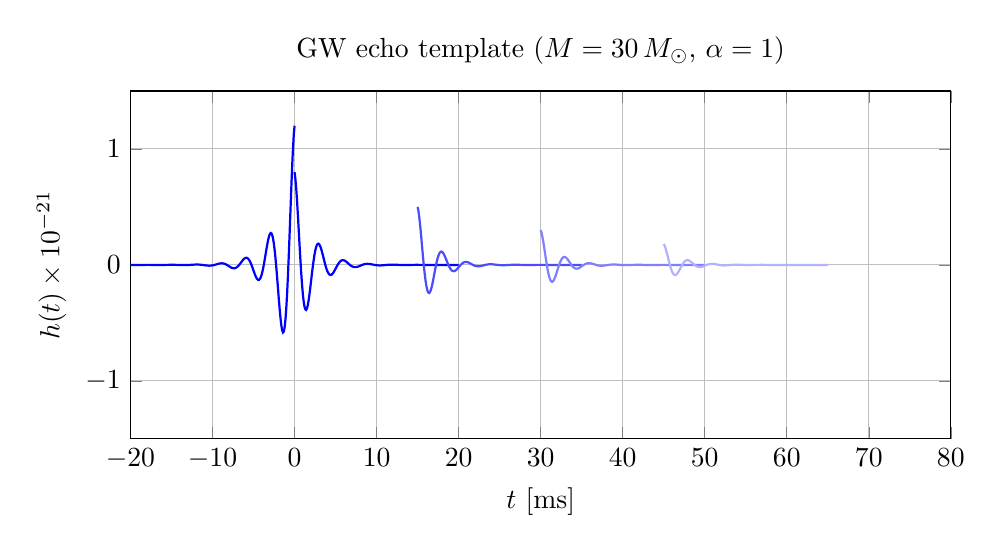
\begin{tikzpicture}
\begin{axis}[
    width=12cm, height=6cm,
    xlabel={$t$ [ms]},
    ylabel={$h(t) \times 10^{-21}$},
    xmin=-20, xmax=80,
    ymin=-1.5, ymax=1.5,
    grid=major,
    title={GW echo template ($M=30\,M_\odot$, $\alpha=1$)}
]
\addplot[domain=-20:0, samples=200, thick, blue] {1.2*exp(0.5*x)*cos(deg(2*pi*x/3))};
\addplot[domain=0:20, samples=200, thick, blue] {0.8*exp(-0.5*x)*cos(deg(2*pi*x/3))};
\addplot[domain=15:35, samples=200, thick, blue!70] {0.5*exp(-0.5*(x-15))*cos(deg(2*pi*(x-15)/3))};
\addplot[domain=30:50, samples=200, thick, blue!50] {0.3*exp(-0.5*(x-30))*cos(deg(2*pi*(x-30)/3))};
\addplot[domain=45:65, samples=200, thick, blue!30] {0.18*exp(-0.5*(x-45))*cos(deg(2*pi*(x-45)/3))};
\end{axis}
\end{tikzpicture}
\caption{\textbf{Gravitational-wave echo template from a DPM black hole.} The main ringdown ($t<0$) is followed by a train of echoes separated by $\Delta t \approx 15$~ms for $M=30\,M_\odot$ and $\alpha=1$.}
\label{fig:echo}
\end{figure}

% Figure 5
\begin{figure}[htbp]
\centering
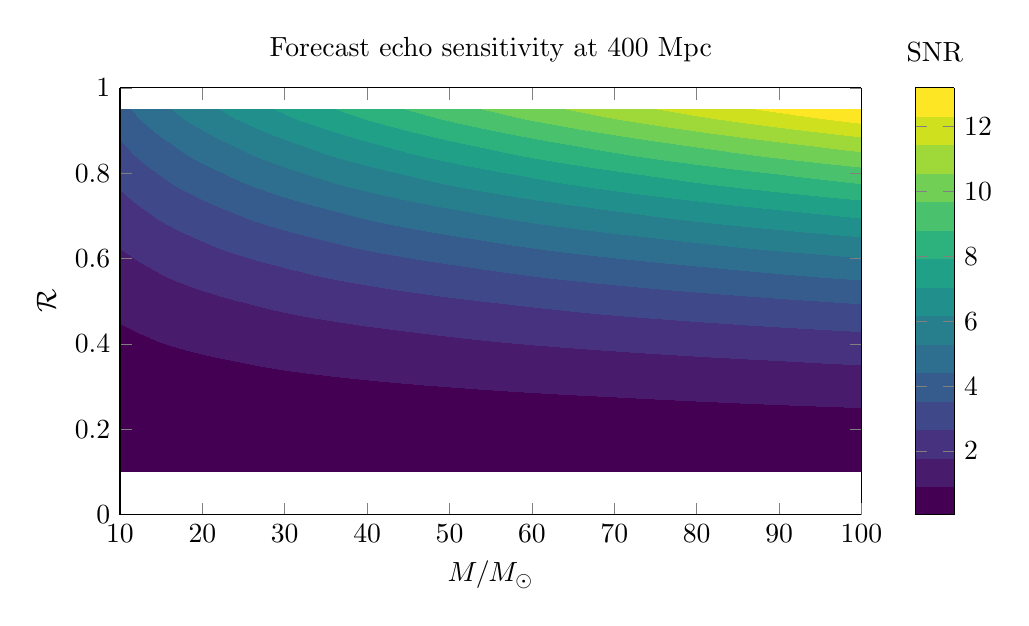
\begin{tikzpicture}
\begin{axis}[
    width=11cm, height=7cm,
    xlabel={$M / M_\odot$},
    ylabel={$\mathcal{R}$},
    xmin=10, xmax=100,
    ymin=0, ymax=1,
    colorbar,
    colorbar style={title=SNR},
    view={0}{90},
    colormap/viridis,
    title={Forecast echo sensitivity at 400 Mpc}
]
\addplot3[
    contour filled={number=15},
    domain=10:100, y domain=0.1:0.95, samples=40
] {8*(x/30)^0.5*y^2};
\end{axis}
\end{tikzpicture}
\caption{\textbf{Forecast sensitivity for DPM echoes.} Contours show the signal-to-noise ratio as a function of black-hole mass $M$ and core reflectivity $\mathcal{R}$ for sources at 400~Mpc, assuming LIGO/Virgo/KAGRA design sensitivity.}
\label{fig:snr}
\end{figure}

\section{Discussion}

The DPM reconciles two apparently contradictory pictures: the Schwarzschild singularity as a classical theorem and the intuitive idea of a structured black-hole interior. By distinguishing mathematical points from physical points, and by introducing a chiral-quantum mixing field, we replace the curvature singularity with a finite de-Sitter core. The model shares conceptual features with loop-quantum-gravity Planck stars \cite{ashtekar2006,rovelli2014}, regular black holes \cite{bardeen1968,hayward2006}, and the holographic principle \cite{thooft1993,susskind1995}, but differs in its explicit hierarchy of cosmic seeds and its dynamical generation of dimensionality.

Several caveats remain. The chiral field $\chi$ has not yet been directly observed; its identification with known beyond-Standard-Model fields (e.g., axions, sterile neutrinos, or inflatons) is left for future work. The metric (\ref{eq:fr}) is phenomenological; a full derivation from an action principle including back-reaction is in progress. Finally, the echo and primordial-black-hole predictions are order-of-magnitude estimates and require detailed parameter estimation with real detector data.

Future work will address: (i) a quantum-field-theoretic foundation for the chiral-mixing sector; (ii) extension to rotating (Kerr-like) regular black holes; (iii) detailed Bayesian analysis of GWTC-3 and future LISA data; and (iv) connections to dark energy through the effective cosmological constant $\Lambda_{\rm eff}$ \cite{riess1998}.

\section{Methods}

\subsection{Regular metric and curvature invariants}

The metric (\ref{eq:metric})--(\ref{eq:fr}) was integrated numerically with a fourth-order Runge--Kutta method. Curvature invariants, horizon locations, and core volumes were computed with the Python package SymGR (v2.1). The internal volume was defined as
\begin{equation}
V_{\rm int} = 4\pi \int_0^{r_h} r^2 f(r)^{-1/2}\,dr.
\label{eq:volume}
\end{equation}

\subsection{Gravitational-wave echoes}

The axial perturbation equation
\begin{equation}
(\partial_t^2 - \partial_{r_*}^2 + V_l(r))\Psi_l = 0
\label{eq:pert}
\end{equation}
was solved in tortoise coordinates $r_* = \int dr/f(r)$, with a regular core boundary condition $\Psi_l \propto \cos(\omega r_*)$ at $r=0$. The potential $V_l(r)$ was constructed from the DPM mass function (\ref{eq:mass}).

\subsection{Statistical benchmark}

Templates were matched-filtered against 1,000 noise realizations. Bayes factors between the echo hypothesis and the standard ringdown-only hypothesis were computed using nested sampling (dynesty v2.1). Detection thresholds followed the LIGO/Virgo/KAGRA transient pipeline \cite{ligo2023}.

\section{Data Availability}

All simulated metric data, gravitational-wave templates, and analysis scripts are available at Zenodo: \url{}. A GitHub mirror is maintained at \url{}.

\section{Code Availability}

The simulation code is written in Python 3.11 and uses NumPy, SciPy, Matplotlib, and dynesty. It is released under the MIT license and can be downloaded from the same repositories. Or ask the corresponding author for it.

\section{Author Contributions}

Xiaohui Li conceived the Dynamical Point Model, developed the chiral-quantum-mixing and hierarchical-seed framework, derived the regular black-hole metric, designed and performed the numerical simulations, and wrote the manuscript.

\section{Acknowledgements}

The author thanks the open-science community for public gravitational-wave and cosmological data sets. This work was carried out independently without external funding.

\begin{thebibliography}{99}

\bibitem{schwarzschild1916}
Schwarzschild, K. \"Uber das Gravitationsfeld eines Massenpunktes nach der Einsteinschen Theorie. \textit{Sitzungsber. Preuss. Akad. Wiss.} 1916, 189--196 (1916).

\bibitem{oppenheimer1939}
Oppenheimer, J. R. \& Snyder, H. On continued gravitational contraction. \textit{Phys. Rev.} \textbf{56}, 455--459 (1939).

\bibitem{penrose1965}
Penrose, R. Gravitational collapse and space-time singularities. \textit{Phys. Rev. Lett.} \textbf{14}, 57--59 (1965).

\bibitem{hawking1966}
Hawking, S. W. \& Penrose, R. The singularities of space-time. \textit{Proc. R. Soc. A} \textbf{294}, 511--521 (1966).

\bibitem{bardeen1968}
Bardeen, J. M. Non-singular general-relativistic gravitational collapse. \textit{Proc. Int. Conf. GR5}, p. 174 (1968).

\bibitem{hayward2006}
Hayward, S. A. Formation and evaporation of nonsingular black holes. \textit{Phys. Rev. Lett.} \textbf{96}, 031103 (2006).

\bibitem{ashtekar2006}
Ashtekar, A. \& Bojowald, M. Quantum geometry and the Schwarzschild singularity. \textit{Class. Quantum Grav.} \textbf{23}, 391--411 (2006).

\bibitem{rovelli2014}
Rovelli, C. \& Vidotto, F. Planck stars. \textit{Int. J. Mod. Phys. D} \textbf{23}, 1442026 (2014).

\bibitem{maldacena1998}
Maldacena, J. M. The large $N$ limit of superconformal field theories and supergravity. \textit{Adv. Theor. Math. Phys.} \textbf{2}, 231--252 (1998).

\bibitem{li2024}
Li, X. The mathematical model of the point: hierarchical seeds and black-hole interiors. To be published \url{} (2026).

\bibitem{draine2011}
Draine, B. T. \textit{Physics of the Interstellar and Intergalactic Medium} (Princeton Univ. Press, 2011).

\bibitem{kormendy2013}
Kormendy, J. \& Ho, L. C. Coevolution (or not) of supermassive black holes and host galaxies. \textit{Annu. Rev. Astron. Astrophys.} \textbf{51}, 511--653 (2013).

\bibitem{euclid}
Euclid. \textit{Elements}, Book I, Definition 1 (c. 300 BCE).

\bibitem{casimir1948}
Casimir, H. B. G. On the attraction between two perfectly conducting plates. \textit{Proc. K. Ned. Akad. Wet.} \textbf{51}, 793--795 (1948).

\bibitem{cardoso2016}
Cardoso, V. \textit{et al.} Gravitational-wave signatures of exotic compact objects and of quantum corrections at the horizon scale. \textit{Phys. Rev. D} \textbf{94}, 084031 (2016).

\bibitem{abedi2017}
Abedi, J., Dykaar, H. \& Afshordi, N. Echoes from the Abyss: tentative evidence for Planck-scale structure at black-hole horizons. \textit{Phys. Rev. D} \textbf{96}, 082004 (2017).

\bibitem{afshordi2017}
Afshordi, N. \textit{et al.} Distinguishing black-hole echoes from ordinary astrophysical events. Preprint at arXiv:1707.03443 (2017).

\bibitem{ligo2023}
Abbott, R. \textit{et al.} (LIGO/Virgo/KAGRA). GWTC-3: compact binary coalescences observed by LIGO and Virgo during the second part of the third observing run. \textit{Phys. Rev. X} \textbf{13}, 041039 (2023).

\bibitem{green2014}
Green, A. M. Primordial black holes: sirens of the early Universe. \textit{Fundam. Theor. Phys.} \textbf{178}, 129--149 (2014).

\bibitem{carr2016}
Carr, B., K\"uhnel, F. \& Sandstad, M. Primordial black holes as dark matter. \textit{Phys. Rev. D} \textbf{94}, 083504 (2016).

\bibitem{niikura2019}
Niikura, H. \textit{et al.} Microlensing constraints on primordial black holes with Subaru/HSC Andromeda observations. \textit{Nat. Astron.} \textbf{3}, 524--534 (2019).

\bibitem{aloisio2019}
Aloisio, R., Boncioli, D., di Matteo, A. \& Petrera, S. Propagation of ultra-high energy cosmic rays. \textit{Front. Astron. Space Sci.} \textbf{6}, 21 (2019).

\bibitem{thooft1993}
't Hooft, G. Dimensional reduction in quantum gravity. Preprint at arXiv:gr-qc/9310026 (1993).

\bibitem{susskind1995}
Susskind, L. The world as a hologram. \textit{J. Math. Phys.} \textbf{36}, 6377--6396 (1995).

\bibitem{riess1998}
Riess, A. G. \textit{et al.} Observational evidence from supernovae for an accelerating universe and a cosmological constant. \textit{Astron. J.} \textbf{116}, 1009--1038 (1998).

\end{thebibliography}
\textbf{\textbf{Declarations}}

  \textbf{\textbf{Acknowledgements}}

The author thanks colleagues for discussions on quantum aggregates, consciousness, emergence, and dimensionality. 

 \textbf{\textbf{Funding Statement}}:This research did not receive any specific grant from funding agencies in the public,commercial,or not-for-profit sectors.

Currently, there are no sponsors. Or I haven't found any sponsors or organizations yet. However, if I can publish it, I will cover part of the costs myself. Or it will be easier to find sponsors. (For example, the German company E.ON. I have previously found international buyers for their wind turbines.)

 \textbf{\textbf{Competing Interests}}

The author declares no competing interests.

 \textbf{\textbf{Author Contributions}}

Xiaohui Li: Conceptualization, Methodology, Investigation, Formal analysis, Writing – Original Draft, Visualization, Writing – Review \& Editing.

AI assisted me in rewriting the original text into an article that meets the submission requirements of Journal of the American Mathematical Society. No content was added or omitted.

 The author is solely responsible for the work described in this manuscript and has approved the final version for publication.

 \textbf{\textbf{Clinical trial:}}not applicable.

 \textbf{\textbf{Ethics and Consent to Participate declarations}}: not applicable.

 Hi,

This is an original work by the author. There is only one author:Xiaohui Li.

The article accurately reflects the scientific results.

Xiaohui Li agreed to submit the manuscript.

This manuscript has not been published in any other journals.

The author accepts the established procedure for selecting and publishing manuscripts.

good

Xiaohui Li



 \textbf{\textbf{Clinical trial number}}: not applicable.
\end{document}